Ud fra ovenstående use case analyser er vi fortsat med at designe en løsning på
opgaven. I lighed med den foregående opgave har vi besluttet os for en løsning
med en decorator, der sørger for at gøre det let at oversætte spillet til et
andet sprog. I vores tilfælde har vi en lidt speciel GUI, der - imodsætning til
en ‘normal’ GUI - afventer en forespørgsel fra vores Gamecontroller/Decorator.
Dette afspejles i vores BCE diagram. I vores BCE diagram er lagt op til en
central controller, hvilket vi dog har valgt at ‘bøje’ lidt i
klassediagrammet.\\
\FloatBarrier
\begin{figure}[h]
\section*{BCE Diagram}
\addcontentsline{toc}{subsection}{BCE Diagram}
\centering
\makebox[\textwidth]{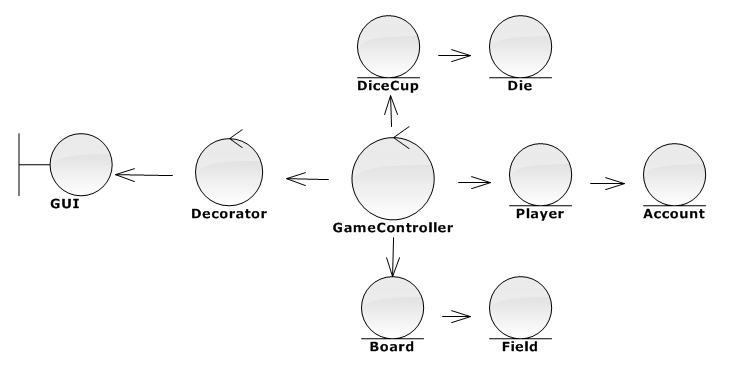
\includegraphics[width=\textwidth]{Robustnessdiagram1}}
\caption{\emph{BCE diagram}: Bemærk den lidt usædvanlige
relation mellem GameController Decorator og GUI. GUI afventer en forespørgsel
fra Gamecontroller/Decorator, hvorfor pilen vender modsat vanlig interaktion med
en GUI.}
\end{figure}
\FloatBarrier
\begin{figure}[h]
\section*{Design Klasse diagram}
\addcontentsline{toc}{subsection}{Design Klasse Diagram}
\centering
\makebox[\textwidth]{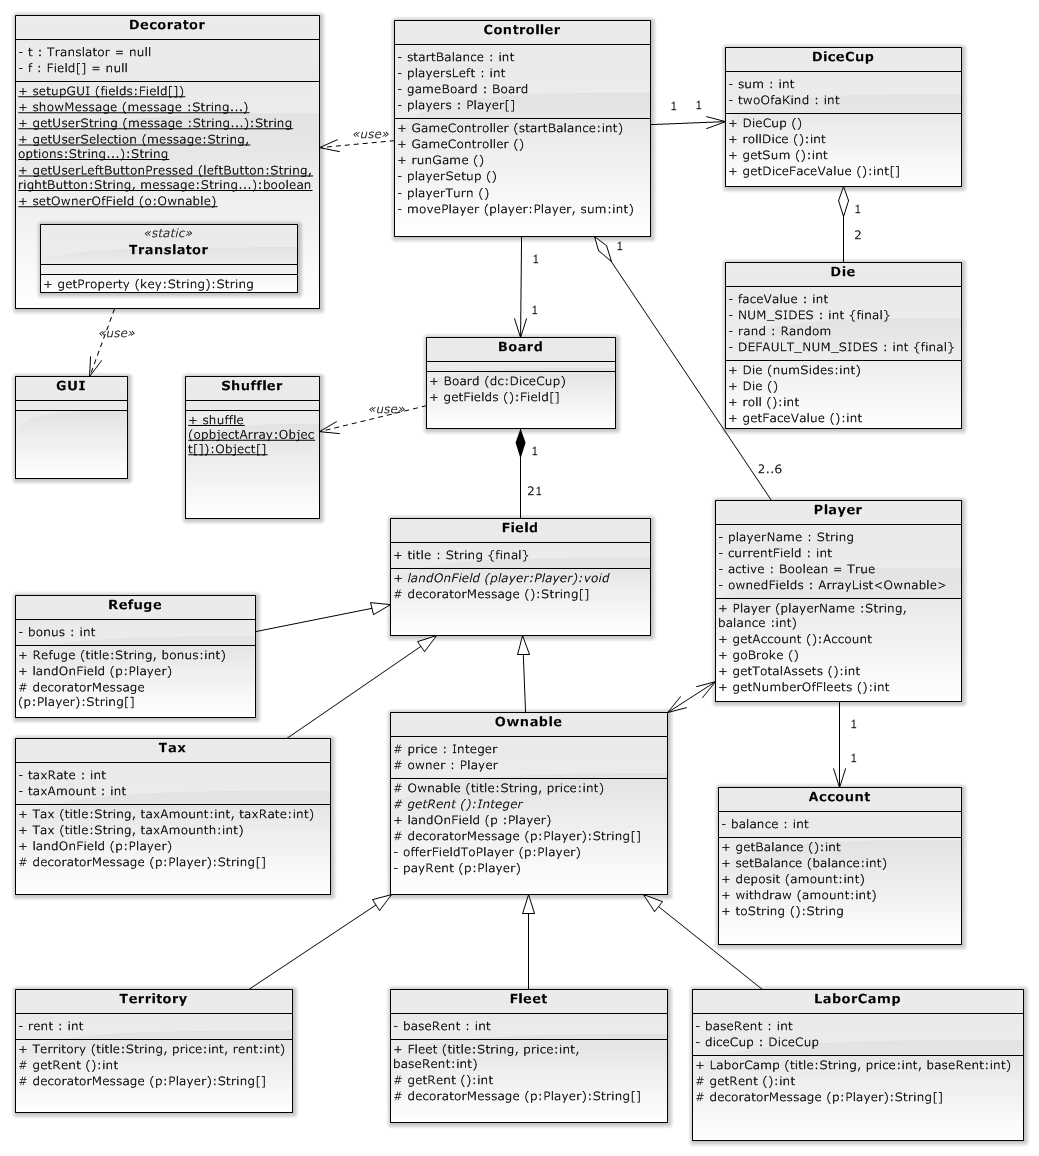
\includegraphics[width=0.8\paperwidth]{Classdiagram1}}
\caption{\emph{Design klasse diagram}: Flere ‘use’ relationer er udeladt for
overskuelighedens skyld. Således er der en ‘use’ relation fra Refuge, Tax,
Territory, Fleet, LaborCamp og Player til Decorator, der er en statisk klasse og
dermed kan tilgås globalt. Desuden er udeladt en association fra LaborCamp til
DiceCup, der bruges til at tilgå terningslaget.\\
I design klassediagrammet har vi udviklet BCE modellen yderligere, så
den rent faktisk afspejler koden. Der er dukket to nye hjælperklasser op - Shuffler og
Translator, der er henholdsvis en statisk hjælperklasse, der kan blande objekter
i et array og en indre klasse, der oversætter Strings via en properties fil,
der er sprogspecifik.}
\end{figure}
\FloatBarrier
\section*{Arv, Polymorfi og Abstract}
\addcontentsline{toc}{subsection}{Arv, Polymorfi og Abstract}
Klassen Field er nu videreudviklet til at have et arvehieraki, der reflekterer
at Fields er forskellige, men har ensartede attributter og metoder - altså
udviser polymorfi. Polymorfi er: \emph{“Muligheden for at bruge den samme kode på
flere forskellige objekter, og for at den kode kan opføre sig forskelligt alt
efter hvilket objekt der er tale om.”}\cite{buildingJava} I vores kode bruger vi
polymorfi til at differentiere mellem forskellige felters landOnField metode, og
vi bruger det i decoratorMessage til at bestemme hvilket text output, der skal
sendes til vores Decorator og videre til GUI.\\
\indent Alle felterne har attributten ‘title’ tilfælles, hvorfor den ligger i
øverste klasse ‘Field’ i arvehierarkiet. Desuden implementerer Field metoden
decoratorMessage(), og en abstrakt metode - landOnField(). Det at en metode er
abstrakt, betyder at den ikke bliver  implementeret i den klasse hvor den er
erklæret abstrakt - det vil sige den ikke  har en metode-body. Fordelen ved at
erklære en abstrakt metode i superklassen er  at man tvinger sub klasser til at
implementere klassen, og man derfor kan være  sikker på at alle subklasser har
metoden. Når en metode bliver erklæret abstrakt  skal klassen også erklæres
abstract. For en klasse betyder dette at den ikke  længere kan instantieres, så
hvis man skal bruge den bliver man nødt til at  nedarve den til en sub-klasse.\\
\indent Ownable er super klasse for de felter  der kan købes - og en sub klasse
af Field. Det er meningsfyldt, da de alle skal  kunne købes - altså har en pris,
‘price’ og en ejer ‘owner’ og skal implementere  metoder til at beregne leje -
getRent().\\
\indent Med de to super klasser Field og  Ownable har vi opnået at kunne
genbruge så meget kode som muligt og undgår  dermed at skulle rette flere steder
i koden når metoderne skal opdateres.\\
\FloatBarrier
\section*{Sekvensdiagrammer}
\addcontentsline{toc}{subsection}{Sekvensdiagrammer}
Ud fra uses cases og klasse diagram har vi forsøgt at analysere flowet i spillet
og modelleret det i de følgende sekvensdiagrammer.
\begin{figure}[h]
\centering
\makebox[\textwidth]{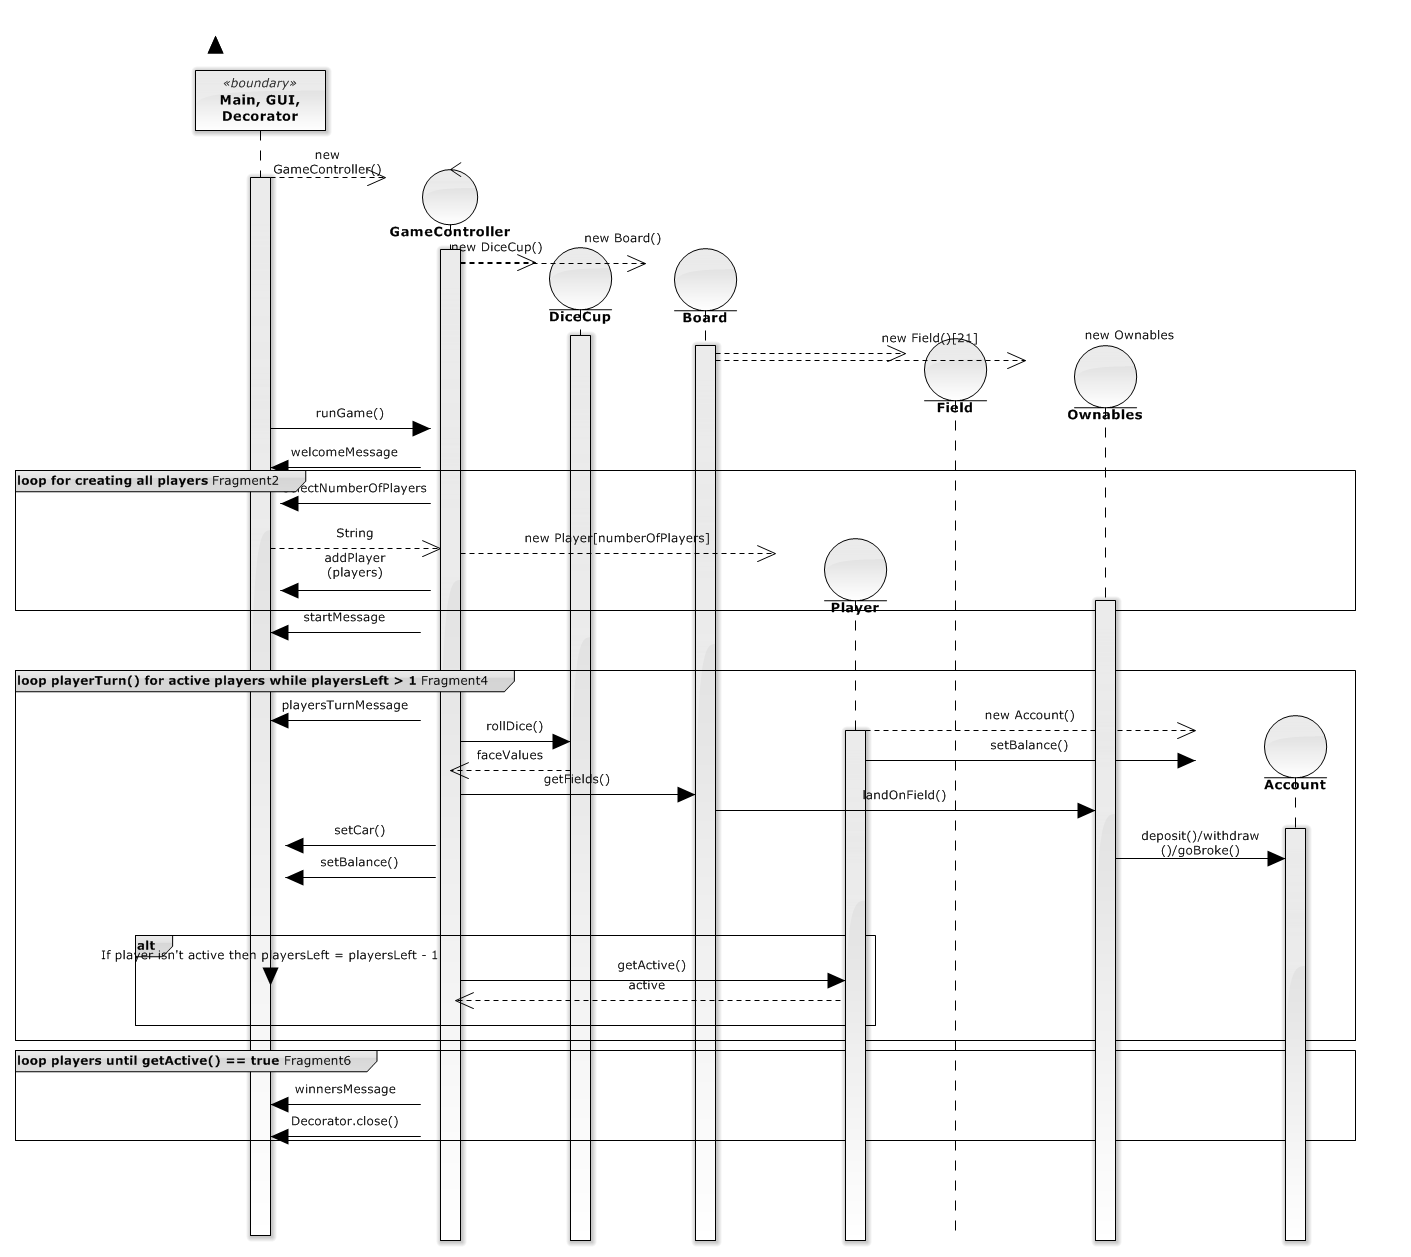
\includegraphics[width=\paperwidth]{DesignSequenceDiagram}}
\caption{\emph{Sekvensdiagram 1}: Play Game.}
\end{figure}
\FloatBarrier
\begin{figure}[h]
\centering
\makebox[\textwidth]{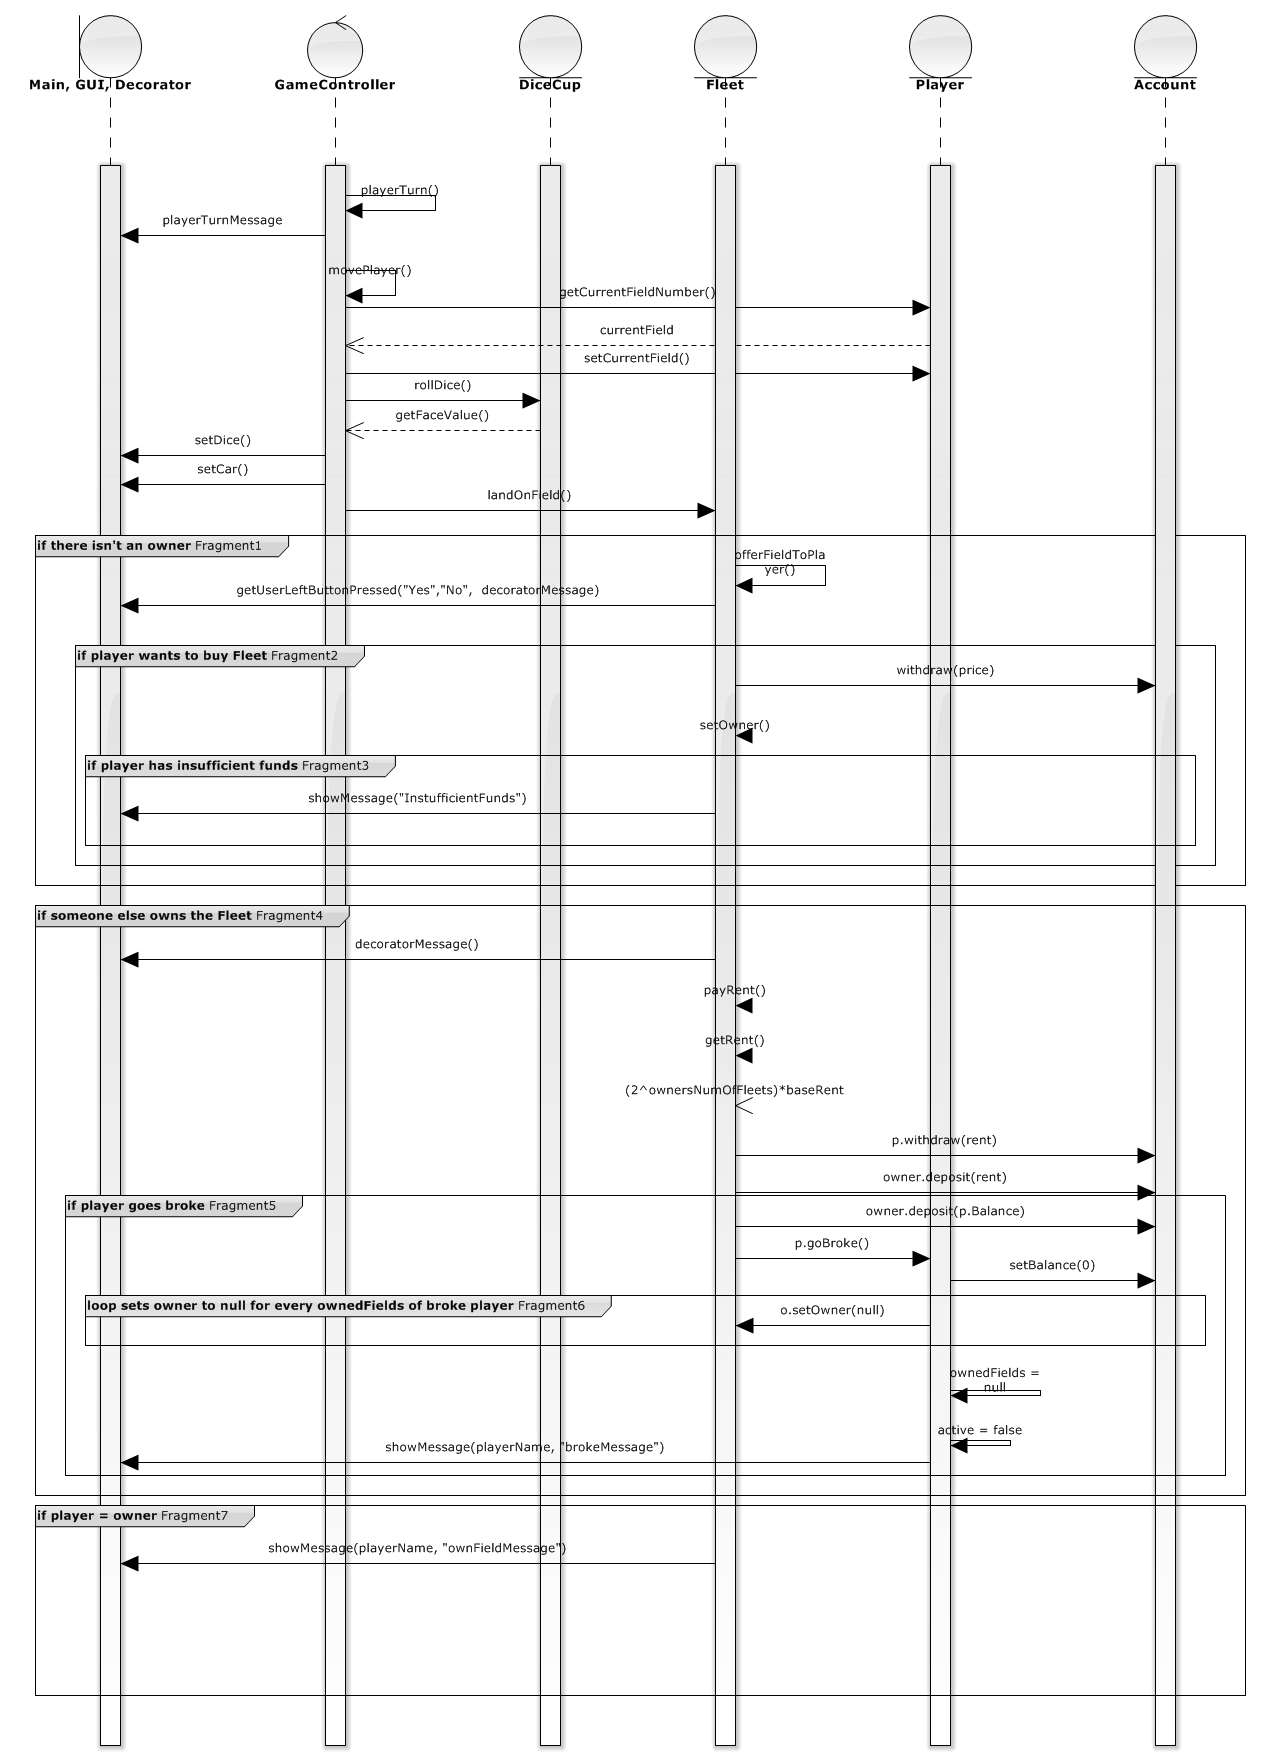
\includegraphics[width={0.8\paperwidth}]{Sequencediagram3}}
\caption{\emph{Sekvensdiagram 2}: Land on Field.}
\end{figure}
\FloatBarrier
Sekvensdiagrammerne er blevet lidt forsimplet for at fremme forståelse, og for
at ikke få for mange metodekald, der ikke ville bidrage til forståelsen af
diagrammet. Klasser der fungerer sammen og/eller ensartet er slået sammen.
Klasser af begrænset vigtighed for diagrammerne er også udeladt. Shuffler
indeholder en statisk metode, der blander felterne i starten af spillet. DiceCup
og Die arbejder så tæt sammen, at Die er undladt. Die er, som navnet hentyder,
en terning. Ownable er en superklasse til alle typer af felter, der kan ejes.
Fields er en superklasse til alle typer af felter. De forskellige typer af
felter, er slået sammen i det første diagram, og er kaldt Ownables, og i det
andet diagram, hvor vi viser landOnFleet, har vi valgt at udelukke de andre
felter, og ladt Fleet være den Ownable vi modellerer, da den er en subklasse af
“Ownable”. Mange returns er også blevet undladt for overskueligheden. Der er
brugt tre forskellige ikoner for klasser, nemlig Boundary, Control og Entity
(BCE), og man kan skelne dem ad ved at Boundary ser ud som, at den rører ved en
væg, Control har en lille pil på sig, og Entity ser ud som den rører ved noget
gulv. Derudover er der brugt to typer kasser. Loops, som repræsenterer loops,
hvis køringspremisser eller formål er beskrevet i den lille tekstboks øverst i
firkanten. Det andet er alt, som er kort for alternate. Dette viser et andet
udfald, der kan ske. Det bliver brugt til at vise ‘if’s og øverst i boksen er
præmissen for det givne if-alternativ anført.\\
\indent Det første sekvensdiagram viser et overordnet forløb af programmet, mens
det andet diagram viser alle de forskellige udfald, der kan opstå, når en spiller
lander på et  felt af typen Fleet. I det første er det på et lidt højere niveau
end i det  andet, da vi i det andet graver helt ind og ser på alle de
forskellige ting, der  kan ske, og ender derved med seks alternate-bokse.\\
\indent Hvis en spiller lander på en Fleet, er der allerede tre muligheder. Hvis
ingen ejer Fleet, skal det tilbydes til spilleren, hvorefter han kan vælge om han vil
købe den eller ej,  men der er en ekstra mulighed i det, at han måske ikke har
penge nok.\\
\indent Mulighed nummer to er, at en anden spiller ejer den. Så skal rent regnes
sammen, flyttes, og vi må se om spilleren er gået fallit. Hvis han er det, skal 
spilleren smides ud af spillet, og hans felter skal frigøres.\\
\indent Mulighed nummer tre er, at han selv ejer feltet, og så skal han bare
have en besked om, at han er landet på sit eget felt.
\section*{GRASP patterns}
\addcontentsline{toc}{subsection}{GRASP patterns}
Vi har forsøgt at arbejde med ‘responsibility driven design’ og implementeret
Controller, Creator, Information Expert, Low Coupling, High Cohesion og
Polymorphism.\\
\indent \emph{Controller} paradigmet er søgt overholdt ved vores GameController
klasse, der håndterer al spil logik og delegerer ansvaret videre. I vores projekt har vi
en lidt speciel statisk GUI, der tillader at vi tilgår den fra alle klasser i
programmet. Da den algoritme som felterne bruger er afhængig af spillerens
input fra GUI’en, har vi skullet vælge mellem at implementere 1) en løsning
hvor GameControlleren først tilgår feltet for at høre om det kan ejes, dernæst
om den kan købes eller er ejet, og dernæst eventuelt sætter ejeren for feltet,
eller 2) som vi i stedet har valgt - en løsning hvor felterne optræder som
subcontrollere og selv tilgår GUI’en for at håndtere hvad netop det felt gør.
På den måde bryder vi bevidst med BCE paradigmet (I det felterne også er
entities), men opnår en mere overskuelig løsning kodemæssigt og da relationen
er en ‘use’ relation med GUI’en øger det ikke coupling væsentligt. Cohesion
bevares også, da det er felterne selv, der logisk set kender reglerne for hvad
der sker når en spiller lander på feltet. Det er muligt at genskabe BCE, ved at
hvert felt får sin egen controller (hvilket ville være Pure Fabrication), men i
det givne tilfælde er det meget begrænset hvad en entity klasse skulle
indeholde, hvorfor vi har valgt at undlade at splitte klasserne op.\\
\indent \emph{Creator} er søgt overholdt ved at de klasser der ‘contains’ eller
‘aggregates’ andre klasser, også har ansvar for at instantiere dem. GameControlleren
instantierer DiceCup, der igen instantierer Die. Ligeledes oprettes Player med
account og Board med Fields. Vores Boundary klasse er et specialtilfælde, da den
er statisk, men initialiseres af GameControlleren, der har hovedansvaret for at
interagere med den.\\
\indent \emph{Information Expert} er søgt overholdt, ved kun at bevare
information og referencer i én klasse - den der er den mest oplagt til at indeholde
informationen. Vi har brudt med paradigmet enkelte steder for at opnå en mere
overskuelig løsning. Således har Gamecontrolleren en integer (playersLeft), der
holder styr på hvor mange players der er tilbage. Denne information er dubleret
fra players, der selv holder styr på om de er med i spillet med deres boolean
active. På samme måde ved både felterne hvem der ejer dem og playerne ved hvilke
felter de ejer. Dette giver desuden en højere coupling - da der er en reference
begge veje - Det giver også en lavere cohesion, da det nu er spredt over to
klasser. Man kan argumentere for at det stadig er logisk, da en grundejer kender
sine grunde og skødet på grunden ligeledes er påtrykt en ejer. Vi gør det under
alle omstændigheder for at opnå en simplere implementering af Fleet, der er nødt
til at vide hvor mange fleets ejeren har. Alternativet er at Fleet skal modtage
en reference til board og iterere over alle felterne for at afgøre hvor mange
fleets ejeren har. Et andet alternativ er at oprette en skødedatabase som kan
adspørges når behovet opstår - det ville svare til GRASP konceptet indirection
(og pure fabrication).\\
\indent \emph{Low Coupling} er opnået ved få koblinger pr. klasse - Dice er
koblet til DiceCup, Account til Player og Fields til Board, der igen er koblet
til GameController (se klasse diagram). GameControlleren har naturligt lidt
højere coupling - da  Dicecup, Players og Board (og Decorator) alle har
betydning for game-flowet. Det  er et acceptabelt antal bindinger - der
understøtter high cohesion. Vi  implementerer en undtagelse med et specifikt
felt - ‘Labor Camp’, der har en  reference til DiceCup. Det er gjort for at
kunne beregne lejen - uden at skulle  passe summen af øjne til feltet. En
alternativ løsning kunne være at  implementere DiceCup som en Singleton, der
kunne tilgås globalt. Som allerede  nævnt har vi en ‘use’ relation fra alle
felttyperne til GUI - idet de tilgår GUI  for at spørge spilleren om han vil
købe grunden eller betale et fast beløb eller  procent af formue i skat. Da det
er en ‘use’ relation er coupling stadig lav.\\
\indent \emph{High cohesion} er forsøgt bevaret ved at klassernes ansvarsområder
er nært beslægtede. Således har Die kun ansvar for terningernes øjne og at ‘slå’ et nyt
tilfældigt slag. Dicecup håndterer summen af øjnene og relaterede opgaver og så
fremdeles. Dette er i høj grad understøttet af low coupling, hvilket også
afspejles i at vi bryder med high cohesion samtidig med at vi bryder med low
coupling i tilfældet med ejerskabet af fields (som beskrevet ovenfor under
information expert)\\
\indent \emph{Polymorphism} er implementeret i vores felter. Her er
ensartede klassers kode forsøgt samlet i superklasser, således at vi genbruger
kode i højest muligt omfang og undgår at skrive den samme kode to gange. Det
afspejles tydeligst i decoratorMessage() metoden, der nedarver i 2 niveau og
sammensætter en ensartet besked til spilleren, sammensat af en besked om hvilket
felt man er landet på (bestemt af Field), en besked der afhænger af om feltet
kan ejes (bestemt af Ownable) og en besked fra selve feltet. Dette understøtter
reusability, idet ændringer i koden kun skal indføres et sted.